\section{Redes Neurais}
\label{sec:redesneurais}

A primeira inteligência utilizada foi a Redes Neurais.

Como pode-se observar a melhor base a ser utilizada em Redes Neurais é a Car, tendo acurácia de 95,73\%, em seguida vem a base Adult e a WPBC com 77,95\% e 77,23\% respectivamente, por último, as bases com menor acurácia foram Abalone e Yeast com 55,68\% e 44,21\% respectivamente. Uma curiosidade é que as bases Adult e WPBC tiveram um desempenho relativamente próximo.

O gráfico abaixo mostra com clareza os resultados de todas as bases com seus valores máximos e mínimos, e claro, sua média para definir qual a melhor.

\begin{center}
      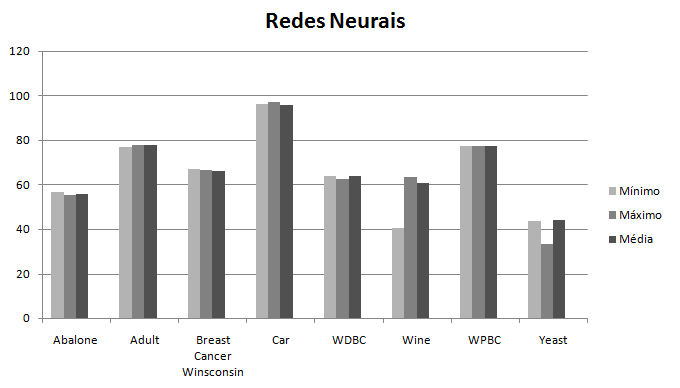
\includegraphics[scale=1.0]{imagens/redesneurais.png}
\end{center}
 
